\documentclass{article}

\usepackage{amsfonts, amsmath, amssymb,color, graphicx, caption}

\title{Practical Motif-Finding in Brain Networks}
\author{Evan Mahone\\St. Mary's College of Maryland}

\newcommand{\rood}[1]{\textcolor{red}{[#1]}} %for displaying red texts

\begin{document}

\maketitle
\newpage

\begin{abstract}
The purpose of the current study was to analyze and improve upon the methodological limits to network motif discovery in brain networks. First, technical details defining brain networks, and their limits are explored. Next, a review of network motif discovery is done. Improvements upon the current best known algorithm are explored, and a new approach to methodology and an algorithm are proposed. Following this a study using the proposed methodology and brain networks of 520 children with and without ADHD is done as proof of concept for the methodology. Finally, the methodology and results are analyzed and the current state of network motif discovery in brain networks is further reviewed. Significant results are found on functional connectivity datasets in the frequency of specific subgraphs between individuals with and without ADHD. Suggestions are made for improvements in methodology and tools used in network motif discovery in brain networks research.
\end{abstract}

\section{Introduction}
.
%%subsection::Network Motifs -- A summary of network motifs 
%%subsection::Purpose -- why did I do this SMP?
In the past 15 years there has been an explosion in the use of graph theoretical techniques in the study of brain networks\cite{bullmore09}. Graph theory, in a broad sense, is the study of distinct elements, \textit{vertices}, and the connections or relationships between them: \textit{edges}. Graph theory has been used in research in Although it is primarily used in math and computer science it has been used in a wide variety of disciplines including economics, sociology, biology, and physics. Graph theory, as a methodology, has been used to expose the computational underpinnings of the brain. Early research showed the ``small-world'' characteristics of the brain \cite{watts98}. This famous study helped put brain networks research on the map. Many other researchers investigated the small-world-ness of the brain networks of different populations, including people with alzheimer's disease \cite{starn07, sanz10, zhao12}, schizophrenia \cite{liou08} and ADHD \cite{wang09}. But thats not all that brain networks research has encompassed - a full review of graph theoretical techniques used in brain network research can be seen in \cite{sporns10}. 

\subsection{Network Motifs}
One graph theoretical measure of a network which has seen a lot of research in biology, but not as much in brain network research is the network motif. A network motif is a pattern found in a network whose occurence is statistically significant in comparison to other networks (usally random) with similar characteristics. Network motifs have been theorized to be computational building blocks of the networks they reside in. For example, in \cite{alon07} Alon describes 6 different types of feedforward loops found in protein interaction networks. In addition, in \cite{sporns04} Sporns describes the difference between a structural and functional motif, where a structural motif denotes the patterns of connections which form in a motif, and a functional motif, which denotes the subpatterns of effect or direction which can occur in a structural motif.\\
Currently available brain network data limits the search for functional motifs, however. Much of what brain network data is available, such as fMRI, EEG, MEG scans does not include any information about which direction information travels in the network (in graph theory terms, this is called an \textit{undirected network}). This is a limit to the technology; current brain scans do not have the temporal resolution to support such information. Although some methodology such as inferring granger causality or directly effecting brain regions with TMS can provide these results, they are not able to at the level which brain scanning technology can produce undirected networks. 
The difference is apparent in the research. Studies of motifs in brain networks have mostly looked at functional motifs \cite[p.107]{sporns10}. As such the research is limited in quantity and in scale. This has been stagnant even with the release of larger and larger datasets such as those available in the human connectome project \cite{biswal2010} and better technology for network motif detection (described in section 4).\\
\subsection{Purpose}
The purpose of the current study was to analyze and improve upon the methodological limits to network motif discovery in brain networks. First, technical details defining brain networks, and their limits are explored. Next, a review of network motif discovery is done. Improvements upon the current best known algorithm are explored, and a new approach to methodology and an algorithm are proposed. Following this a study using the proposed methodology and brain networks of 520 children with and without ADHD is done as proof of concept for the methodology. Finally, the methodology and results are analyzed and the current state of network motif discovery in brain networks is further reviewed. 
%How graph theory has been used in the past 15 years in brain network analysis introduction to the fundamental concepts of this paper: brain networks, graph theory and network motifs. A description of the purpose of the SMP
%%subsection::Network Motifs
%%subsection::Purpose --why did I do this SMP?

\section{Terminology}
The \textit{order} of a graph is the number nodes it contains. The \textit{size} of a graph is the number of edges it contains. Two nodes are said to be \textit{connected} if an edge exists between them. The \textit{degree} of a node is the number of edges the node makes with other nodes.\\
A graph $H$ is a \textit{subgraph} of another graph $G$ if $V(H)$ is a subset of $V(G)$. A graph $J$ is an \textit{induced subgraph} of a graph $G$ if $J$ is a subgraph of $G$, and $J\neq G$.
A graph $G$ is \textit{isomorphic} to another graph $H$ if $G$ and $H$ have the same order, and are connected in the same way. That is, a bijection $b$ exists from $V(G)$ to $V(H)$ such that $uv\in E(G)$ if and only if $b(u)b(v)\in E(H)$. The bijection $b$ is called an $isomorphism$. An \textit{isomorphic class} of graphs is a collection of graphs which are all isomorphic to eachother.\\
An \textit{automorphism} of a graph is a shuffle of it's nodes such that an isomorphism exists from the original graph to it's shuffle. It should be noted that a concatenation of automorphisms is also an automorphism. A trivial automorphism exists as well - which is the automorphism in which no nodes move. An \textit{automorphism group} for a graph $G$ is the set of node shuffles (including the trivial shuffle) which produce a graph isomorphic to G.\\

\section{Brain Networks}
	Brain networks are characterized by different measures of brain connectivity. Brain connectivity is a broadly defined term for physical, statistically significant, or causal relationships between neural units or regions. There are three major types of brain networks based on 3 categories of connectivity. 
\subsection*{Connectivity}
	\textit{Structural brain networks} are the simplest of the three categories conceptually. These networks are based on \textit{structural connectivity} - which can refer to how neurons or neural regions are physically connected to one another. Networks of neurons and neuronal processes, traced in vitro, such as the neuronal network of the hermaphrodite Caenorhabditis elegans \cite{white86} are examples of structural brain networks. Regional networks might consist of a map of statistical relationships between morphological characteristics of the brain. These networks are found using imaging or tracing techniques which get a static picture of the brain such as DTI \cite{iturria07,iturria08} or structural MRI \cite{lerch06}.\\ 

	\textit{Functional connectivity}, the basis of \textit{functional brain networks}, consist of statistical relationships in time-series data of brain activity in anatomically distinct neural regions. Numerous functional brain networks have been assembled from both resting state \cite{van10} and task based \cite{rissman04,koshino05}fMRI data, PET \cite{friston93}, EEG \cite{lowe98, joudaki12}, and MEG \cite{stam09} scans.

	\textit{Effective connectivity} and \textit{effective brain networks} are an extension of functional connectivity. It differs from functional connectivity in that causality or direction is known between nodes in the network. This is akin to saying that effective brain networks are directed graphs. 

\subsection{Constructing Graphs from Brain Networks}
	%STRUCTURAL 
	Diffusion tensor imaging (DTI) is a method which allows for the assessment of the diffusion of water through open areas in the brain. When fibers are more organized, water diffuses through them with greater ease than when the fibers are randomly distributed. It is a measure of the restriction of the diffusion of water through tissue, which is measured by Fractional Anisotropy (FA) and diffusivity. Higher FA and lower diffusivity indicate a greater integrity of the tissue that is being looked at, which in turn gives a good estimate of whether an area of the brain is part of a tract. There are two approaches to DTI: the voxel-wise approach and tractography.\\
	In the voxel-wise approach you look at the whole brain, and look for places that are significantly different on FA or diffusivity. This tells you where there are differences in the brain. 
	In tractography you use predefined brain atlases to define the regions (tracts) in which to record. You then compare the levels of DA and diffusivity to discover which tracts have a greater connection. A brain network derived from DTI data would look different depending on which technique you used; thought both would be weighted structural networks. In the voxel-wise approach your networks nodes would be voxels - the smallest region of space a DTI can read. Edges would represent statistical relationships between voxels; how different they measure. As such this type of network would be an abstract one. It would not correlate exactly with physical connections in the brain. If the tractography approach was taken, nodes would be the predefined region in the brain atlas. The edges in the network would be a function of FA and diffusivity recorded between the two regions. 
	
	%FUNCTIONAL
	%fMRI
	When a region of your brain is active there is a delayed response of blood flow to this region. This is called the hemodynamic response and the blood oxygen level dependent (BOLD) signal is a measure of this. Changes occur in the magnetic structure of blood when it is depleted of oxygen. Thus an MRI scanner can detect changes in the activity of a brain region.
	A resting state fMRI evaluates connections and interactions between brain regions across time in an individual who is not assigned a specific task (at rest). Resting state fMRI also uses the BOLD signal. Often the BOLD signal is recorded at brain regions specified by brain atlas - based on anatomical parcellations of the brain. In doing this you can get a measure of the strength of functional connections between regions. Task-based or event-based fMRI measures the same in an individual who is performing a specified task. The BOLD signal is also measured in task-based fMRI. In task-based fMRI the BOLD signal may be contrasted against different tasks or points in a time-series. A brain network developed from either resting state or event-based fMRI would be a functional brain network. It would have brain regions from the brain atlas as nodes. Connection weights would be values calculated from the intensity of BOLD signals in conjunction with a measure of how close in time BOLD signals were recorded for adjacent nodes. 
	
	%EEG/MEG 
	EEG records electrical activity of the brain along the scalp. Generally it is a measure of electrical activity that is a function of neuronal activity. With a basic EEG you put electrodes on the scalp. There are different spectra (distributions of activity) which fluctuate over time. Different types of waves are categorized by their frequencies. Evoked potentials are derivatives of EEGs and they look at the activity of the brain immediately after an event (usually an outside stimulus). Different frequencies indicate a different level of activity in a brain region. MEG is another form of measurement of electrical activity in the brain. It is a technique for measuring the magnetic fields that result from electrical activity in the brain. It has a better spatial resolution than EEG but cannot reach deeper brain regions. A brain network derived from EEG or MEG data would be a functional brain network. Nodes in a graph representing this network would be brain regions which the EEG nodes are set to record. Edges would be a value representative of how close in time activation recorded by EEG is in one region is to another. 


\section{Network Motif Discovery}
%A description of the current results in network motif discovery. What has been discovered in general, and what discoveries have been made in brain networks? A description of the current problems in network motif discovery. Description of types of algorithms. First a description of Nauty and then bliss.
%%Subsection:: Network Motifs of the Brain
%%Subsubsection:: Motifs in Weighted Networks
%%Subsection:: Network Motif Algorithms
%%Subsubsection:: The Problem of Motif Discovery
%%Subsection:: G-Tries
\begin{figure}[t!]
\includegraphics[scale=.07]{figs/subgraphs.png}
\centering
\caption{Potential motifs: sets of order 3, 4, and 5-connected subgraphs}\end{figure}
Network motif discovery essentially follows 3 steps:
\begin{itemize}
\item{Census of subgraphs on original network}
\item{Census of subgraphs on similar random network}
\item{Statistical evaluation of significant motifs}
\end{itemize}
Pedro ribeiro \cite{ribeiro11}, in detailing the short history of network motif discovery algorithms, puts network motif discovery algorithms into two categories: \textit{Network-centric} and \textit{subgraph-centric}. In network-centric approaches, all possible subgraphs of a network are found, afterwards, isomorphism tests are done between graphs to count the frequencies at which each queried subgraph occurs. In subgraph-centric models, a query of the frequency of each subgraph is done on the network. A detailed analysis of different algorithms which use these models is given in \cite{ribeiro11}. Below I will describe the G-Tries algorithm, which, according to analysis done in \cite{ribeiro11} performs an order better than all other algorithms. A comparison of the G-Tries algorithm with the rand-ESU algorithm, which seems to be the next best performing algorithm \cite{li12} is done on the brain networks used in \cite{rubinov10} as well as the neuronal network of the C. elegans, recently revised in \cite{varshney11}. 
\subsection{G-Tries}
The G-Tries algorithm consists of three parts:
\begin{itemize}
\item{Canonical labeling}
\item{Construction of a G-Trie}
\item{Subgraph census}
\end{itemize}
In the G-Tries algorithm, a tree is constructed which is used as a data structure for the subgraph census. Each node of the tree represents a different subgraph, with parent nodes of a current node as connected subgraphs of that current node. As well, the current node is also a connected subgraph of each of its child nodes. The tree, known as a G-Trie (figure 2) for graph-retrieval is constructed using Ribeiro's own canonical labeling algorithm: GTCanon. A canonical labeling is a way of representing a graph such that any graph which is isomorphic to it will have the same canonical labeling. It the GTCanon function, this presents itself as a transfomation on a graphs indexed vertices represented by an array of indexes telling the graph how to swap its vertices in an adjacency matrix to produce the canonical form of that matrix. In the G-Tries algorithm, the canonical labeling also ensures that earlier nodes in a tree have the maximum degree possible while still holding the properties described above. In this way, the G-Trie is constructed in order to have the least possible number of nodes. All of these properties allow the G-Tries algorithm to optimize over its subgraph census.\\
The GTCanon algorithm begins with another canonical labeling algorithm. Ribeiro has chosen \emph{nauty}, which is described in the next section. This pre-canonical labeling is designed to ensure that a graph census can occur on graphs on which GTCanon fails to fulfill the 3 properties described above. So a graph sent into the GTCanon algorithm is converted to canonical form first. After that, a map of the degree of each of it's vertices is made. The algorithm procedes across every position in the previously described transformation array until it is filled, startin from its end, labeling vertex indices which have filled the array thusfar. The algorithm chooses a next label in the following way. The next vertex index in the transformation array must be one which has not yet been added to the array, and the removal of this vertex must not produce a disconnected graph (this ensures that each subgraph in the G-Trie is connected). Out of the remaining candidates to label, the chosen vertex must have the minimum degree with unlabeled vertices out of all of the unlabled vertices. If a vertex index has still not been chosen, the vertex with the minimum degree with all unlabeled vertices plus the last labeled vertex is chosen. If a vertex index is still not chosen, the vertex with the minimum degree with all vertices is chosen. After this, there seems to still be a chance to fail to choose a vertex. Ribeiro suggests to default to making use of the nauty labeling at this point. The author of this paper interprets this as meaning to apply a specific rule at this point which will always ensure a choice, and the choice will always be the same for canonically labeled graphs, such as choosing the vertex with the minimum index. After a new index is chosen to add to the transformation array, the process is repeated until the transformation array is full. The result is an array of indices where the $i$th index tell us where the $i$th vertex will be shifted to in an adjacency matrix.\\
After this, a G-Trie is constructed in the following way. Take the set of subgraphs you want to perform a subgraph census on, apply the GTCanon function to them and iteratively insert them into your G-Trie, which should initially consist of a a root, with no nodes on it. The leaves of this G-Trie should eventually consist of each of the subgraphs you are censusing. The insertion process goes as follows. At each step you add a portion of of a row of the graphs adjacency matrix to the next node, and advance to that node. The portion of the adjacency matrix that you add are the first $k+1$ values of the kth row of your matrix, where $k$ is the depth of the current node. This tells you that the first $k$-indexed vertices of your graph are the same as the child nodes $k$-indexed nodes. If the portion of the adjacency matrix is the same length as the order of the subgraphs you are censusing, you know that you have reached the end of the tree, you add the last portion of the adjacency matrix, and move on to the next subgraph. If not, you look at all of the children of current node, and look at the portion of the adjacency matrix stored there. If it is the same as the $k+1$ values in the $k$th row of the matrix, you advance and store the $k+1$ values in the $k$th row at the new node. Afterwards, a new child is created, at the current node with the $k+1$ values in the $k$th row in the matrix stored on it. The child node becomes the current node, and this process is done recursively until leaf nodes are found for each subgraph. This construction makes a tree which allows for matching of subgraphs in an optimized number of steps.\\ 
The subgraph census is done by taking a node from the graph we are censusing. At each step in the process we add a neighbor to our current subgraph and advance a level in our G-Trie to the node which matches our current subgraph. We know that this exists because each level of the G-Trie corresponds to an order, and contains every kind of connected subgraph for that order at each level. We keep adding neighbors until we get to a leaf node, at which point we know that we have found one of the subgraphs we are censusing, and we add a count to the frequency count for the subgraph. To ensure that the same graph is not found twice the G-Tries algorithm checks for automorphisms using the \emph{nauty} algorithm. This will not be described in the current paper, but as described later, makes up a large part of the time complexity of the algorithm.\\
The current study suggests the use of the GTries algorithm for the speeds that were reported in \cite{ribeiro11} as well as its potential use in an algorithm described in section 6.
\begin{figure}[b!]
\centering
\includegraphics[scale=.25]{figs/gtrie.png}
\caption{A G-Trie containing order 4 connected subgraphs}
\end{figure}



\section{Graph Isomorphism}
%An analysis of the use of graph isomorphism algorithms in the G-Tries algorithm. 
%%Subsection:: Nauty
%%Subsection:: Current results in graph isomorphism
%%Subsection:: Bliss
The proven isomorphism testing toolkit \emph{nauty} is used on two occasions in the \emph{G-Tries} algorithm: in the canonical labeling portion of the construction of the G-Trie, and the testing for automorphisms in the subgraph query portion of the algorithm. As explained in \cite{li12}, A significant portion of the runtime of the \emph{G-Tries} algorithm relies on testing for isomorphism. Although \emph{nauty} is said to run near linear time \rood{cite} on most input graphs, when the number of input graphs itself is \rood{polynomial, exponential?}
For these reasons the current study also analyzed the performance of different canonical labeling and automorphism-testing software in the context which the \emph{G-Tries} algorithm uses \emph{nauty}. First, the algorithm behind \emph{nauty} is described. Next, a review of the current state of isomorphism-testing algorithms is done. And finally, one of the newer graph isomorphism testing algorithms, \emph{bliss}, is described. 
\subsection{Graph Isomorphism Terminology}
A \textit{graph partition} is a set of subsets (called \textit{parts}) of the nodes of a graph $G$ such that no two elements in the same part connect via an edge. A graph partitioning is also called a \textit{coloring} where parts are called \textit{colors}. A partition with total ordering is an \textit{ordered partition}. A \textit{Trivial part} is a part with only 1 node, \textit{discrtete partition} is a partition with only trivial parts, and the \textit{unit partition} is the partition with only one part - which is simply the set of nodes of $G$. A \textit{color-degree vector}\cite{marchetti11} is a vector for a node $x$ in a graph $G$ with an ordered partition $\pi$ whose $i$th element represents the number of neighbors $x$ has in the $i$th part of $\pi$. An orderered partition $\pi$ is \textit{finer} than an ordered partition $\tau$ if every part of $\pi$ is contained in a part of $\tau$ and every earlier part of $\pi$ is contained within an earlier part of $\tau$. An ordered partition $\pi$ is \textit{coarser} than $\tau$ if it is not finer. An \textit{equitable ordered partition} is an ordered partition, $\pi = {V_1, V_2, \dots, V_m}$ such that for every pair of indices $i$ and $j$, there is a non-negative number $b$ such that the part $V_{i}$ shares exactly $b$ neighbors with $V_{j}$.

\subsection{Nauty}
From 1980 up until the last decade, McKay's algorithm for canonical labeling of graphs \cite{mckay81} had been the fastest known canonical labeling algorithm. This algorithm is found in the nauty package released by McKay. As well, it is one of the most popular algorithms for canonical labeling. There are three strands of nauty, as described by \cite{hartke09}. The first uses propogation of degree information from neighboring nodes. The second uses artificial symmetry to build a search tree whose leaves are isomorphic to the graph we are looking at. The third 
looks at automorphisms in the described search tree. 

\textbf{Degree propogation.} In the first part of McKay's algorithm, nodes of our graph are partitioned, and nodes which are in the same part are compared by degree. The algorithm involves finding the \textit{coarsest equitable refinement} of our graph. 
You begin with a graph and an ordered partitioning (specifically the unit partition). Iterate through the parts, starting with the first ordered part, and ending with the last part.For each part, $V_i$ ,check if each node has an identical color-degree vector. If not, further partition $V_i$ to maximal sized parts with the same color-degree vertex in each part. Order said parts by the degree they make with other parts (starting with the smallest), and replace $V_i$ with this ordered partition. Continue with this until you get through all of the parts of your partititon. At this point, you should have an equitable refinement of the graph. Further strands of the algorithm procede to turn this into the coarsest euqitable refinement of the graph. 

\textbf{Search tree.} McKay's algorithm procedes by creating a search tree with our current equitable ordered partition $\pi$ at the root. Thi Ts portion of the algorithm takes up the largest portion of its time complexity\cite{darga04}. The algorithm goes through each part of $\pi$, and splits the part by an arbitrary node. Child nodes of $\pi$ are the resulting equitable ordered partitions. This process is carried out on child nodes until a discrete ordered partition is found. Thus the leaves are discrete ordered partitions. Importantly, search tree nodes also contain the sequence of arbitrary nodes chosen in the splitting process thusfar. Also importantly, each leaf is an isomorph of our original graph $G$. The tree is generated depth-first.

\textbf{Automorphisms.} The final step of the algorithm is pruning the search tree. This step is done during the generation of the search tree. As proved in \cite{mckay81}, if we discover a node $v_2$ which contains an automorphism from $v_1$ (which is already explored) to itselft, we can automatically discard any nodes which would be children of $v2$. automorphism - we can automatically discard any further generated nodes which contain. Further the same can be done for a node which contains a permutation of other nodes, forming an automorphism. 

\section{Other Algorithms for Graph Isomorphism}{
	Below is a brief outline of the different graph isomorphism algorithms which have been developed in the past decade or so. This discussion was cut short due to time constraints, but a full review can be found in \cite{mckay13}. 
	A number of different algorithms which solve the same problem have been developed since 2004, when \emph{saucy} \cite{darga04} was introduced. \emph{saucy} is very similar to the way that \emph{nauty} is written, except that it is optimized on sparse, ordered graphs of the type developed by conjunctive normal form generating algorithms. \emph{saucy} improves upon the nauty algorithm in the partition refinement procedure. Specifically, the number of 
}

%McKay's algorithm is a depth-first search through maximally refined partitions of a graph. 

%Nodes which can be swapped in an automorphism have the same degree, and their neighbors, and neighbor's neighbors have the same degree. If two nodes have differing degree they can not be swapped in an automorphism. 

%Refinement is used to distinguish vertices which cannot map to eachother in an automorphism. Thus we color the vertices based on their degree...
%If a node has a different degree into another part of the partition, then it can be distinguished among nodes in its part. 

%At each step in the search tree generation a vertex is chosen and is given a new color. 

%Search begins with an initial coloring. From the current node, determine the target color-class: the smallest "ordered" partition that is of order greater than 1. Choose an arbitrary node, and make this into a trivial part (singleton color-class). So if we had $\pi$ as a partition, we now have $\pi'$. Put the new color-class at the end of our ordered partition. Now take $\pi'$ and apply the vertex refinement algorithm to it. 

%%Concluding remarks.
As G-Tries can be reused for multiple analysis, the canonical labeling portion may be negligible except in the case of extreme subgraph sizes. The real portion where the G-Tries algorithm is bogged down is in the automorphism testing \cite{li12}. A study of how different algorithms would perform on this portion of the G-Tries algorithm is discussed in the discussion. It optimizes using the fact that sparse graphs have very few connections to other nodes. Thus, in \cite{darga04} they conclude that fewer child nodes be generated in the partition refinement portion of their algorithm. They achieved a significant speedup on sparse graphs in comparison to nauty. This algorithm may be a good choice as a replacement for nauty in the G-Tries algorithm in order to optimize over brain networks, as brain networks are sparse. Another algorithm which is designed for canonical labeling and has recieved large speedups over \emph{nauty} is \emph{bliss} \cite{juntilla07}, which has shown to have better performance on large and sparse graphs over \emph{nauty}.
%An analysis of the use of graph isomorphism algorithms in the G-Tries algorithm. 
%%Subsection:: Nauty
%%Subsection:: Current results in graph isomorphism
%%Subsection:: Bliss

\section{The ReG-Trie Algorithm}
Before the ReG-Tries algorithm is described, it should be noted that a conceptual error was made in the construction of the algorithm, making it completely unusable for it's intended purpose. Below is a description of the algorithm as it was originally envisioned. A discussion of how to fix the algorithm is described in the discussion section. 
The ReG-Trie algorithm is essentially an extension of Pedro Ribeiro's G-Tries algorithm. It differs, however, in its application. ReG-Trie is designed for the specific use over sets of networks which consist of many of the same connections. More specifically, ReG-Trie was designed to be optimize performance of network motif discovery on weighted networks which have had a range of thresholds applied to them. The algorithm takes advantage of the GTrie structure in order to know the precise outcome on network motif frequencies when an edge is removed.\\
The algorithm uses the exact construction of a G-Trie in Ribeiro's algorithm, the only place where it differs is in the subgraph census step. In the subgraph census, connectional matrices are put in order so that whenever we add a node to our current subgraph, we know exactly where that edges it makes exists on each of the thresholded connectional matrices. The matrices should also be a arranged such that greater thresholded matrices are on the ``bottom'' and less thresholded matrices are on the ``top''. The G-Tries algorithm is run on the ``top'' matrix. Whenever a node is added to our current subgraph, we sequentially poll where each edge occurs on each thresholded matrix. If we meet a matrix which is missing one of the edges we have added on a higher level matrix, we know something about this subgraph, particular to this matrix. The first thing we know is that we do not advance to the same branch which the higher level matrix advances to. If none of the connections from the higher matrix are present, we know that we don't advance at all on the branch. If the higher matrix has advanced to a leaf, we know that that on the lower matrix, and all matrices below that matrix, we do not count this subgraph.\\ 
This is where the conceptual error was made. It had been assumed that knowing a connection is not present means that our lower matrices will not be able to reach a leaf node. This, however, is only the case if we know that a \textit{node} is not present rather than an edge.\\
What this algorithm should have provided was a way for the number of subgraph censuses to be reduced to one for networks which are sequentially derived from eachother by removing edges. Because we would have known that for any missing edge we find, all matrices below the currently-being-checked matrix are also missing that edge, we would have been able to eliminate a number of future computations at least equal to the number of connections removed betwen connections. This however, is surely not the casee. 

%Why the algorithm? Why is your approach to network motif discovery on weighted networks better? Description of the algorithm. Expected uses. 
%%Subsection: Measuring weighted 

\section{Methods}
\subsection{ReG-Tries Implementation}
The ReG-Tries algorithm was first written in R. This choice was made for a few reasons. 
\begin{itemize}
\item{R has a wide range of graph theory, and brain networks related packages readily available. Many of these are packaged with the \emph{igraph} package.}
\item{R provides easy visualization of data. }
\item{Dependency issues. Many of the implementations of graph isomorphism algorithms have not been updated since the papers describing the algorithms were written. Thus many of them are dependent upon older software, and as a result, suffered dependency issues. On the other hand, the igraph package in R has graph isomorphism testing algorithms and canonical labeling (using \emph{bliss}) out of the box.}
\item{R functions as a scripting language, allowing easy data manipulations and prototyping}
\end{itemize}
In other words, R was chosen in order to provide a quick proof of concept, and easy integration for the purposes of this paper. 
There are several costs to choosing R to program the ReG-Tries algorithm. Unfortunately, this was not able to come to fruition.
%Negatives to choosing to program this in R.



\subsection{Data}
In recent years, projects have been developed to release large  brain connectivity datasets, called \textit{connectomes} to the public. Two notable projects are the 1000 functional connectomes project, and its successor the human connectome project. In the current study five hundred twenty functional connectivity matrices and 27 structural connectivity matrices were taken from the UCLA Multimodal Connectivity Database \cite{jesse11} which is part of the Human Connectome Project. The 520 functional connectivity matrices were taken from the ADHD200\_CC200 data set, which contains resting state fMRI connectivity data from 190 individials with ADHD (74 inattentive, 7 hyperactive/impulsive, and 109 combined subtypes) and 303 typically developing children between the ages of 7 and 21. Additionally, the scans were divided 208 by 3012 in the ratio of girls to boys. The 27 structural connectivity matrices were taken from the NKI\_Rockland data set. This set consisted of DTI tractography data from ``normal subjects,''. The structural connectivity datasets were later dropped from the analysis because of time constraints. 

\subsubsection{Processing}
The original matrices were weighted and undirected. Each connection matrix in the ADHD200\_CC200 data set had 190 vertices defined where each vertex corresponded to a predefined brain region. The ADHD200\_CC200 was obtained through the seeding method, so each edge is an estimate of the connection strength between predefined brain regions. The NKI\_Rockland connection matrices each had 188 vertices defined, where each represented a predefined tract region. Edges represented estimates of the densities of tract regions. 
In order for the connectivity matrices to be used for network motif discovery three steps were taken. Each connectivity matrix was processed using R (version 3.0.0). First, the data was normalized so that all values were between 0 and 1, where 0 would represent no connection, and 1 was the ``heaviest edge'' in the matrix.  Second, weak connections were removed according to thresholds. For functional connectivity data, an absolute threshold,  \ $t_{\alpha}$ between the values of 0 and 1 was applied, such that every value in our matrix below $t_{\alpha}$ would be removed. Third, the remaining values were binarized - that is - connections which were removed were converted to zeroes and remaining connections were converted to ones. These matrices could now be called undirected unweighted adjacency matrices: blueprints for undirected graphs. As such they were now suitable for analysis of network motifs.\\
\subsubsection{A unique approach to analyzing undirected motifs}
In the literature, as described by \cite{rubinov10} and exemplified by studies like \cite{deuker09} and \cite{wang09} only one prespecified threshold is applied to connectivity matrices to get unweighted data. This poses a problem, as graph theoretical measures are thus dependent on that one threshold. This is especially apparent as many of these studies cite previous studies on their decision of threshold - which makes both studies dependent on that threshold. The methodology of applying a range of thresholds has been suggested in the footnotes of \cite{sporns10}, but not used in research to this authors knowledge. Analysis can then be done on what properties are present in each of the thresholds - telling use what measures are present in the most highly connected portions of our network, and what properties are present only in specific networks. It is clear that properties held across multiple thresholds prove to be more present properties, and thus a stronger argument for their existence is gotten.\\
The use of multiple thresholds should provide a unique character to the network motif as well. Analysis of which motifs break down across the thresholds and which are still present gives us a more informative idea of the strength of a motif than at least one current method for producing weighted network motifs. In \cite{onella05}, Onella describes a technique for recording the \textit{intensity} of a network motif in a weighted network. Intensity is a measure of the average of all edge weights in a subgraph. What the problem with this is is that if a certain subgraph consistently has 1 edge which is heavily weighted, this will skew the whole motif to be labeled as more intense. With the methodology proposed here - if we look across increasing thresholds - we can give an estimate of where the connections are lost. We look at which motifs have decreased in frequency between thresholds, and which have increased in frequency. If we see, for example, a high frequency of pentagon subgraphs in one threshold, but see more path subgraphs on 4 vertices, we may be able to make an assumption - with other variables held constant that connections were lost from the pentagons between thresholds. This would provide a better character for the strength of a subgraph.\\
In the current study, 6 thresholds where 15, 30, 45, 60, 75, and 90\% of the weakest connections were removed were applied to each connectivity matrix (seen in figure 3).  
Because the ReG-Tries algorithm was never completed, analysis of motifs was done using the GTrieScanner software developed by Pedro Ribeiros (http://www.dcc.fc.up.pt/gtries/) on all connected subgraphs of order 3 and order 4 (see figure 1).
\begin{figure}
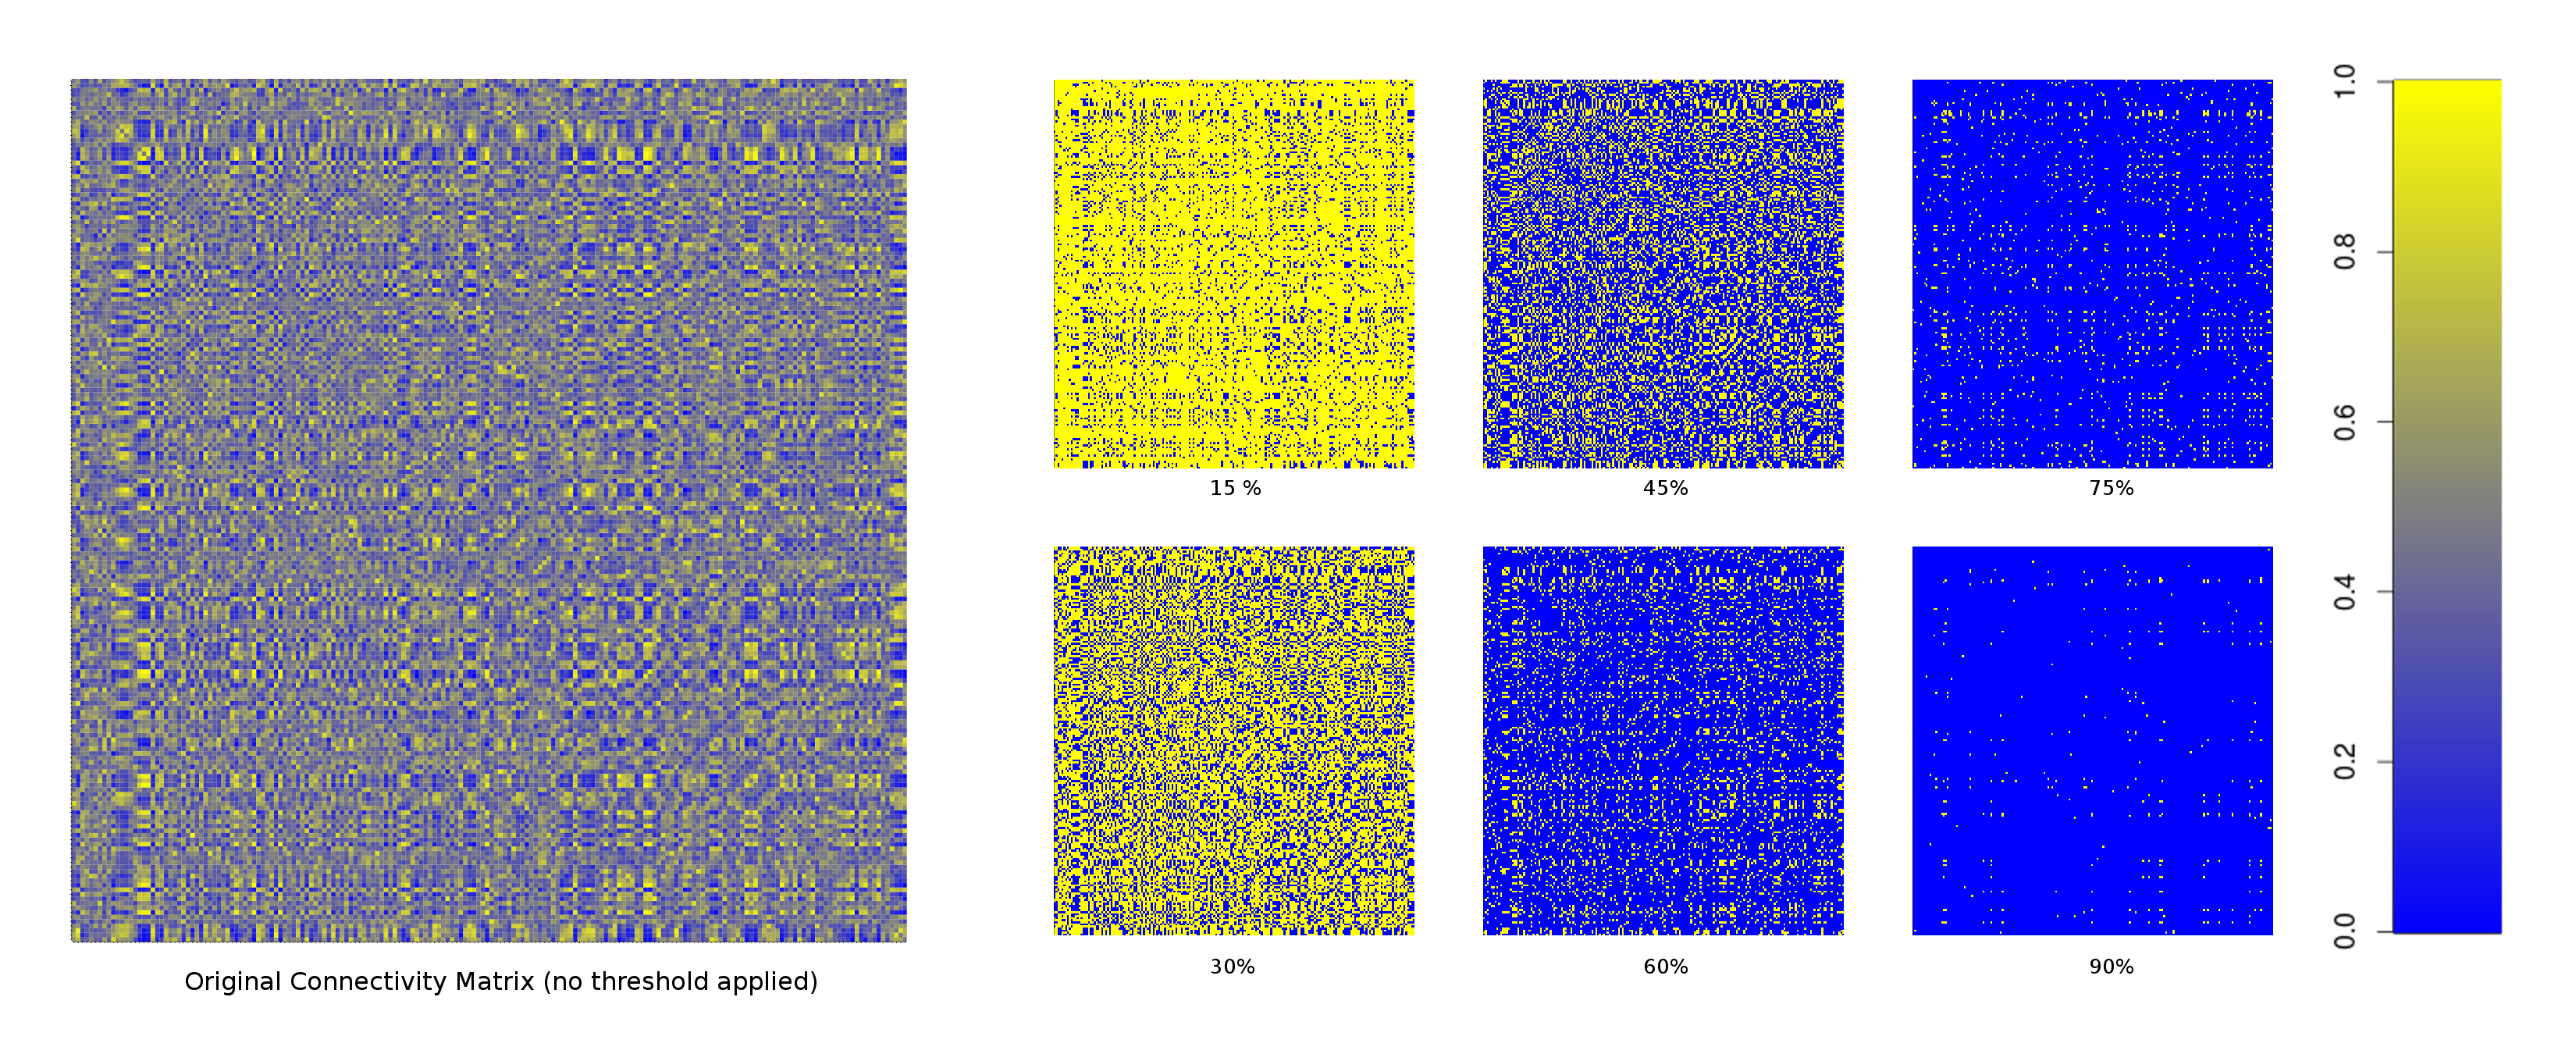
\includegraphics[width=\textwidth,height=\textheight,keepaspectratio]{figs/matrices.png}
\caption{A weighted connectivity matrix (left) with 6 thresholds applied to it (right).}
\end{figure}

\subsection{Comparison of Graph Isomorphism Algorithms}
Analysis of the performance of different graph isomorphism algorithms was originally planned as part of this study, but was never completed. A plan for a future study which follows through is described in the discussion. 
%First: a general outline of the methodology. The development of the algorithm is described. Then the process of data collection 
%%Subsection:ReG-Tries Implementation
%%Subsection: Data
%%Subsubsection: 


\section{Results}
Statistical analysis was done using the SPSS statistical analysis package v.19 and statistical programming language R version 2.15.1. Statistical significance was evaluated at p=.05. 
\begin{figure}
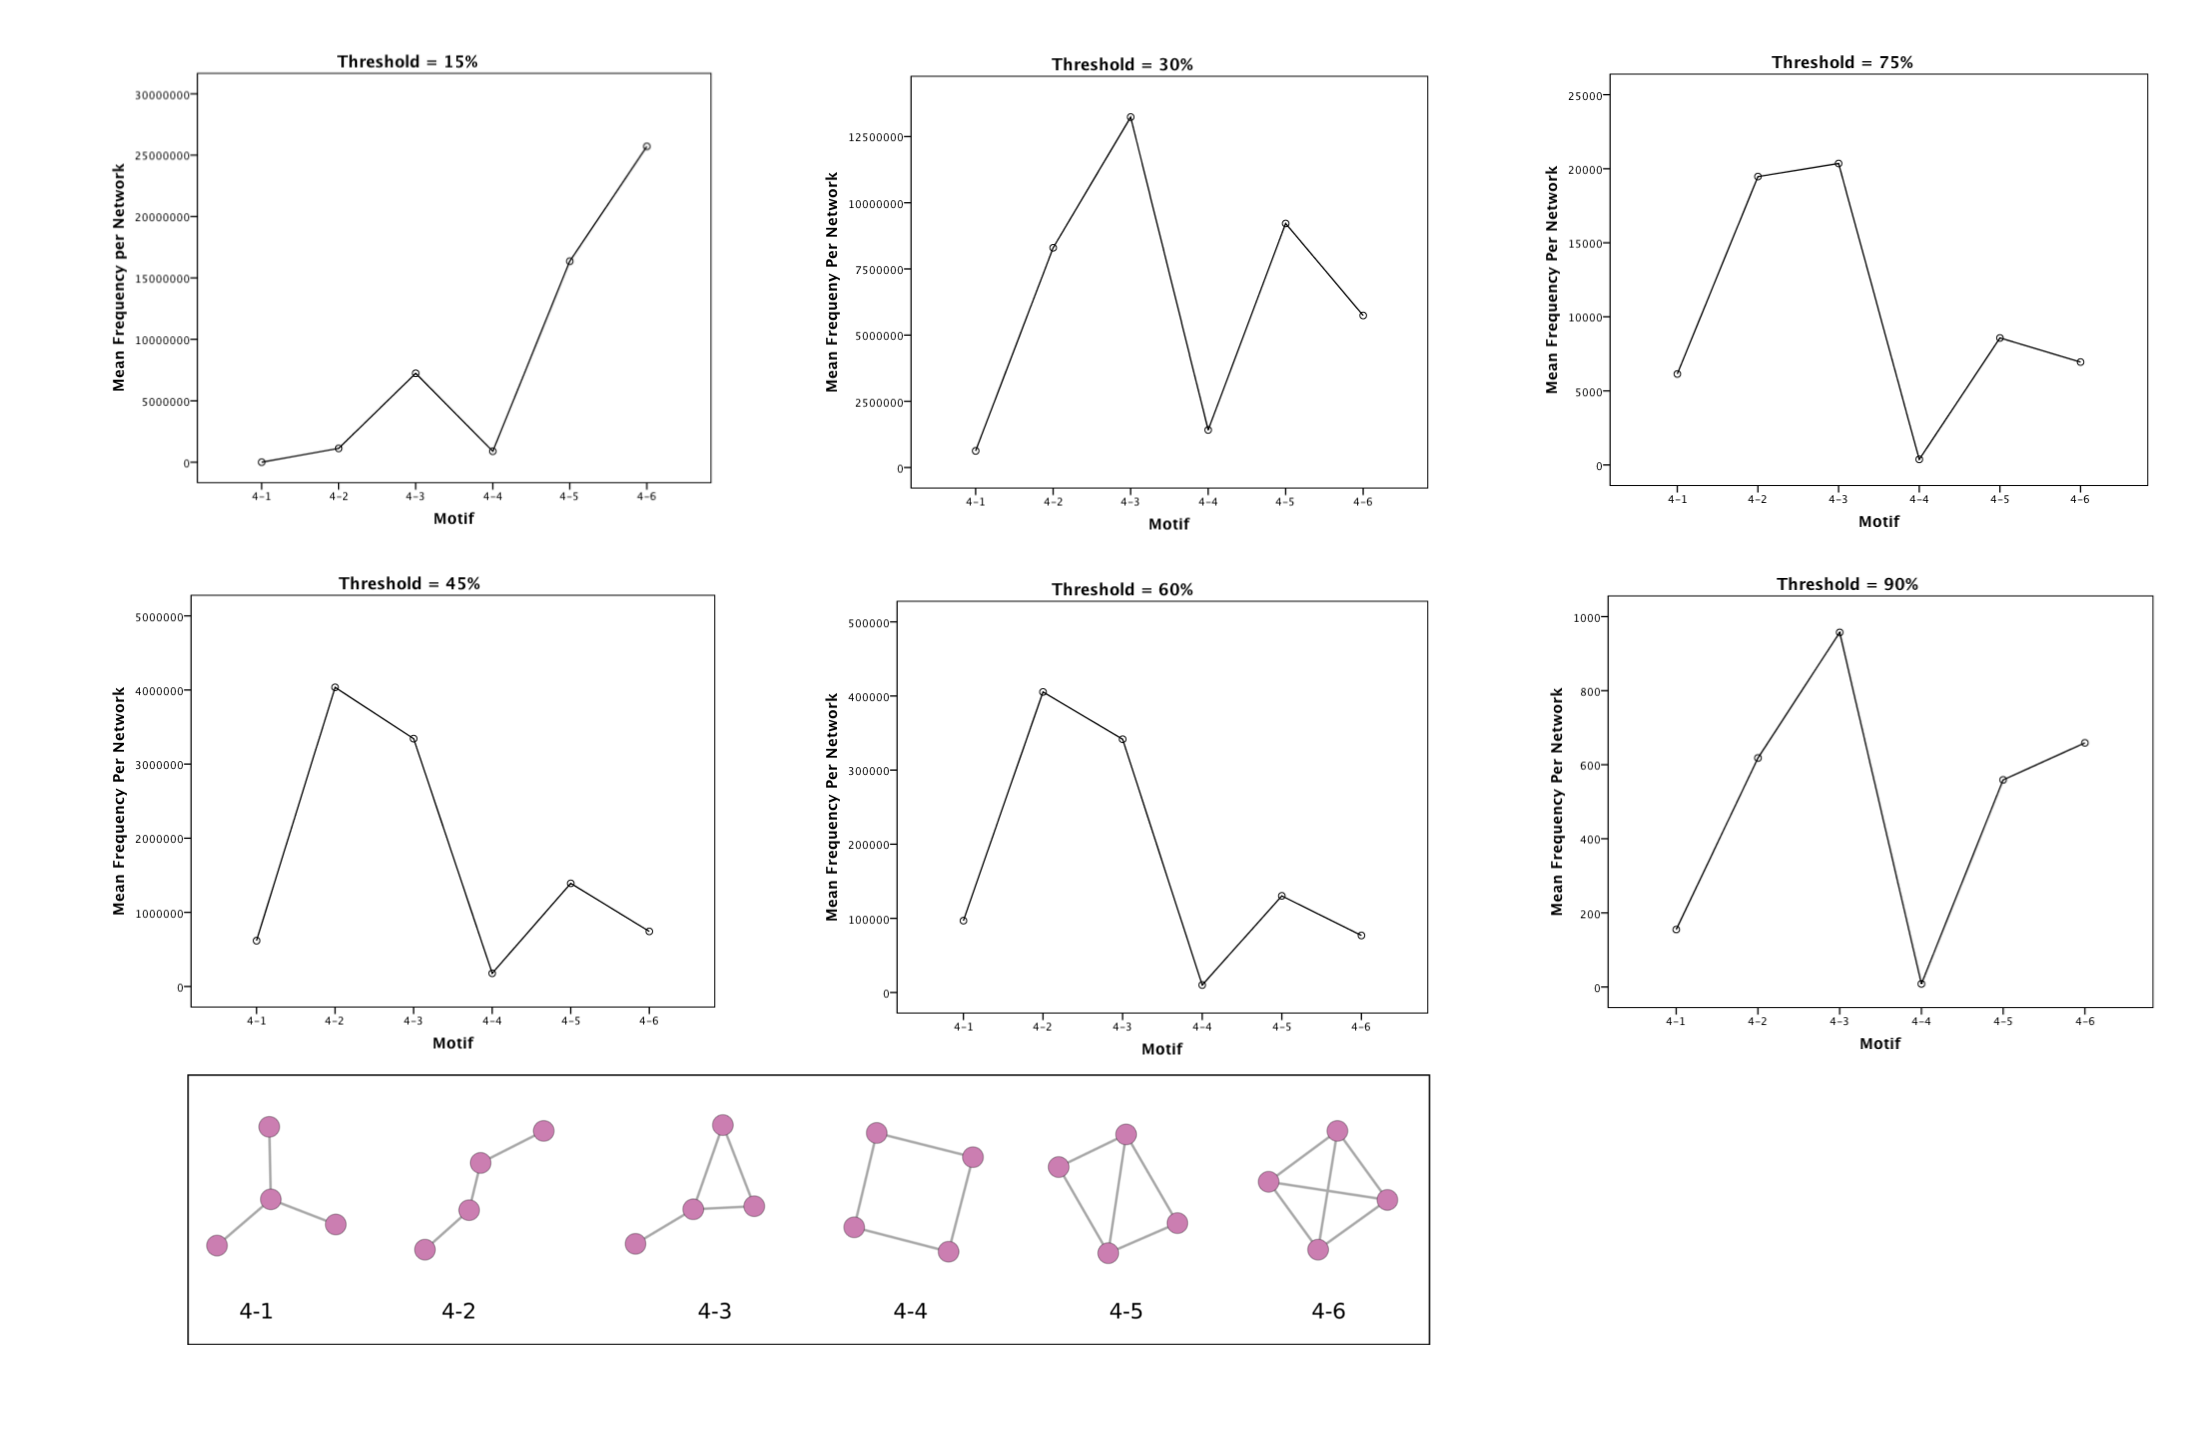
\includegraphics[width=\textwidth,height=\textheight,keepaspectratio]{figs/motif1.png}
\caption{Mean subgraph frequencies by threshold}
\end{figure}

\begin{figure}
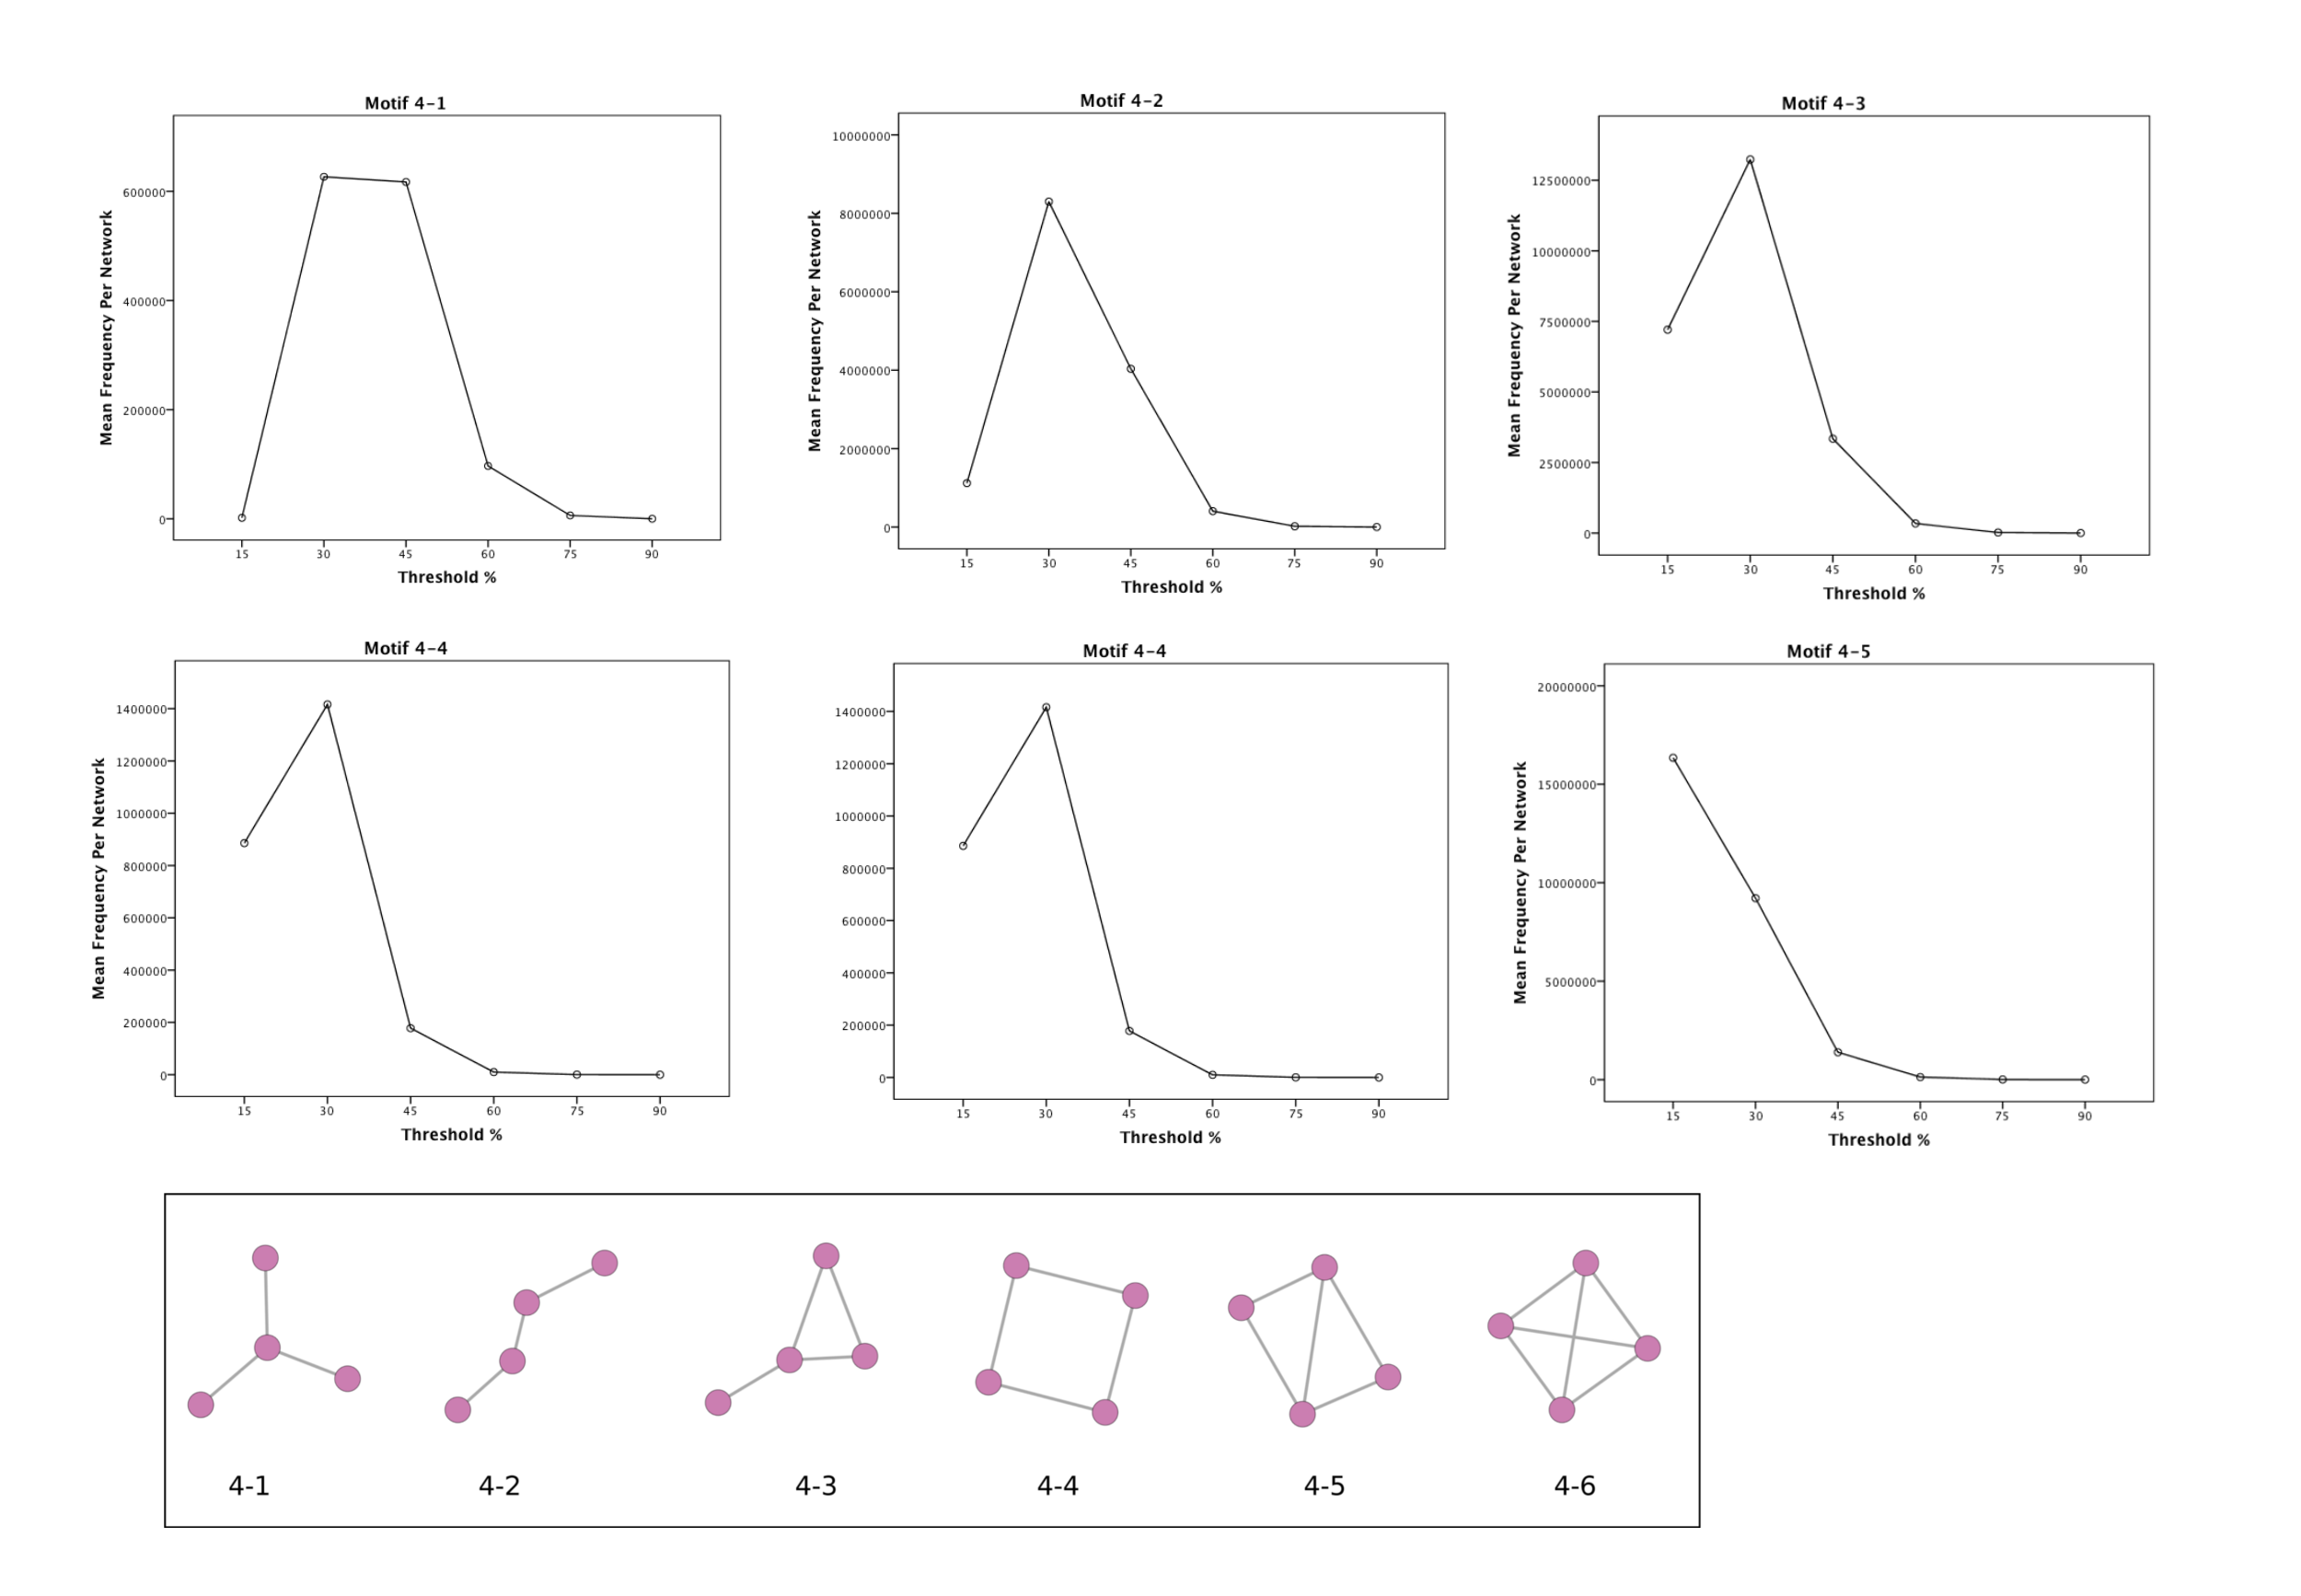
\includegraphics[width=\textwidth,height=\textheight,keepaspectratio]{figs/motif2.png}
\caption{Mean subgraph frequencies by motif}
\end{figure}

\begin{figure}
\caption*{Table 1: Significance Levels for Group Comparisons (ADHD vs. Control) of Mean Frequencies per Network, by Motif and Threshold.}
\begin{center}
\includegraphics{figs/table1.png}
\end{center}
\end{figure}
The 60\% threshold was the only threshold in which significant group differences ($p < .05$) were detected. The 60\% threshold was the most sensitive to group differences between ADHD and control for Motifs 4-2, 4-3, 4-5, and 4-6. Typically developing individuals were found to express less (mean = 394128.5, sd =108528.6) of graph 4-3 than individuals with ADHD (mean = 425151.5, sd = 170217.4, $p < .012$), they also saw less of subgraph 4-3, (mean = 325311.7, sd = 148836.6), (mean = 369994.5, sd = 228788.2, $p < .007$), subgraph 4-5 (mean = 121089.7, sd = 83884.94), (mean = 146333.6, sd = 136222, $p < .009$) and subgraph 4-6 (mean = 64072.93, sd = 73167.64), (mean = 99157.56, sd = 224300.3, $p < .009$). The 90\% threshold was the most sensitive to group differences for Motifs 4-1 and 4-4, however the results were not statistically significant.\\
No signigicant patterns were found across thresholds, however, a more thorough analysis might reveal more.\\
Additionally, an analysis comparing the performance of the GTrieScanner algorithm against the ESU algorithm found that results were not significantly different for most brain network datasets. However, on the C. Elegans neuronal network, GTrieScanner performed at a level more than 10 times greater than the rand-ESU algorithm. Results are shown in 
\begin{figure}
\caption*{Table 2: Comparison of GTrieScanner and Rand-ESU algorithms.}
\includegraphics{figs/gtries-esu.png}
\end{figure}

\section{Discussion}
\subsection{Results of Subgraph Analysis}
A significant difference was found in the expression of 3 different motifs in the resting state fMRI connectivity of individuals with ADHD against typically developing individuals. Comparable thresholds on similar datasets were not able to be found in the research. However, the greater frequency of these subgraphs in particular might be reflective of research suggesting that brain networks of individuals with ADHD lie more on the ordered side of the small-world network spectrum than random \cite{wang09}. This is further supported by the fact that both the present study and cited study look at resting state fMRI connectivity matrices. Further research and analysis must be done to be conclusive, however.\\
Additionally, it is apparent that 4-cycles are statistically under-represented across all thresholds of data, making the 4-cycle an antimotif. In an intuitive sense, this may be because the 4-cycle lies between more sparse structures such as 4-1 and dense structures like 4-4 or 4-5. Its lack of occurence may also be an effect of the small-world character of brain networks, where random connections are likely to disrupt the perfect order of the 4-cycle.\\
Further analysis of the data may reveal other significant patterns between thresholds. However, the current author is not equipped with a knowledge of how to perform this analysis correctly. 
\subsection{Future Plans}
\subsubsection{Comparison of Graph Isomorphism Algorithms}
In the future, the GTrieScanner source code could be modified to output the specific graphs that were sent into the nauty algorithm for automorphism queries, across a number of different networks. This way, we know exactly the types of graphs that the automorphism testing in the G-Tries algorithm must be optimized for. Each set of graphs would be held seperately, so that the computational time for each network with a different algorithm can be tested. We could pass each of sets of graphs into another algorithm such as \emph{Bliss} and we would record the total running time on the set. The total running time would be compared across the different networks. 
\subsubsection{Corrections to ReG-Tries algorithm}
The Re-GTries algorithm was not successful due to a conceptual mistake made by the author. However, the concept of the algorithm still may be salvageable. The ReG-Tries algorithm would have been viable if one was able to predict which subgraphs a motif decomposes into when it loses an edge. It is possible to predict the subgraph which will occur when removing a \textit{node} from our motif via the G-Trie, which gives us a sequence of subgraphs our motif is composed of. The decomposition concept of The ReG-Tries algorithm thus might still be useful in areas of research like single-node motifs \cite{echtermeyer11} or neuronal death - like that experienced in Alzheimer's disease. Another approach would be to reorganize the way in which the G-Trie is organized to allow us to have deterministic knowledge of the edges present in a motif. For example, we can know that if we currently have a cycle, if we remove any edge from that cycle we know that we will have a path. As well, for any k-connected motif, removal of exactly one edge will always produce graphs in the same isomorphic class. Is there a way that we could optimize the G-Trie to build on these types of graphs, which give us definite knowledge of the edge structure of the graph? And would this pseudo-G-Trie be able to perform anywhere near the speed at which the G-Tries algorithm performs, or be able to perform at all? 
\subsubsection{Further analysis of Motifs on the ADHD200 set}
It would be interesting to see if the overabundance of certain order 4 subgraphs in the brain networks of children with ADHD would present themselves as higher frequencies of related 5 order subgraphs. The calculation of all measures on the 520 datasets took a total of 2 hours of computation. Given the results reported here of GTrieScanner on the C. Elegans neuronal network, 5 order subgraphs also seem viable. 

\section{Conclusion}
%Summarize what was learned. 
%Summarize the results.
%Future Plans
%What I did wrong
%%Subsection: Improvements to ReG-Tries
%%Subsection: Reflection on St. Mary's Project
\subsection{The Current State of Network Motifs in Brain Networks}
The current paper revealed methodology for discovering and analyzing network motifs in large brain networks. The GTries algorithm performed adequately in network motif detection on 520 individuals across 6 thresholds - making it a viable algorithm for motif discovery in brain networks, especially given its reported running time. Suggestions were made to further improve the GTries algorithm specifically in the realm of brain networks research. Current algorithms in graph isomorphism seem to outperform those used in the GTries algorithm, however, successful implementation would be needed as proof. A novel methodology in studying network motifs in brain networks was used in the current study, which revealed a significant difference in the distribution of 4 order subgraphs in functional brain networks of individuals with ADHD versus those without. This provided a proof-of-concept for the methodology. 
\subsection{St. Mary's Project Reflection}
There are many things that I wish I had done early on during my St. Mary's Project experience that would have helped out in the long-run:
\begin{itemize}
\item{Narrowed down on a topic early}
\item{Toned down my ambition}
\item{Collaborated with my SMP advisor}
\item{Set deadlines for myself which I knew I wouldn't be able to keep}
\end{itemize}
As a result of these missteps, I ended up spending a dispropportionate amount of my time researching what I should do for my SMP. This occured until this semester, which very much made even later missteps I made hurt much worse. Were I to repeat my SMP, I would definitely \textit{not} let myself choose my own topic. Rather, I would have my advisor instruct me the entire way. Because I chose a topic that was not an area my SMP advisor had expertise, nor was it a topic which anyone at the school had expertise in, I took it upon myself to become my own advisor on the matter, which ended in me turning in my SMP late. Overall, I have a lot of regrets about how I handled myself on this project, and I wish that I had realized the self-defeating cycle I would be getting myself into - and stopped doing things according to my schedule. At this point in time though, I am just really really glad that I am finished. 
%Summarize what was learned. 
%Summarize the results.
%Future Plans
%What I did wrong
%%Subsection: Improvements to ReG-Tries
%%Subsection: Reflection on St. Mary's Project

\bibliographystyle{plain}
\bibliography{bibliography}

\end{document}